% Gemini theme
% https://github.com/anishathalye/gemini

\documentclass[final]{beamer}

% ====================
% Packages
% ====================

\usepackage[T1]{fontenc}
\usepackage{lmodern}
\usepackage[size=custom,width=100,height=75,scale=1.0]{beamerposter}
\usetheme{gemini}
\usecolortheme{labsix}
\usepackage{graphicx}
\usepackage{booktabs}
\usepackage{tikz}
\usepackage{caption}
\usepackage{pgfplots}
\usepackage{array} % for spacing tables out \extrarowheight
%\pgfplotsset{compat=1.15}

% ====================
% Lengths
% ====================

% If you have N columns, choose \sepwidth and \colwidth such that
% (N+1)*\sepwidth + N*\colwidth = \paperwidth
\newlength{\sepwidth}
\newlength{\colwidth}
\setlength{\sepwidth}{0.04375\paperwidth}
\setlength{\colwidth}{0.275\paperwidth}

% Spacing / Formatting
\newcommand{\separatorcolumn}{\begin{column}{\sepwidth}\end{column}}
\newcommand{\itembox}[1]{\item {\makebox[10cm]{#1 \hfill}}}

% Standard Probability
\DeclareMathOperator{\E}{\mathbb{E}}
\newcommand{\PP}{\mathbb{P}}
\newcommand{\RR}{\mathbb{R}}

% Data-Consistent Inversion Framework

\DeclareMathOperator*{\param}{\lambda}
\newcommand{\pspace}{\Lambda}
\newcommand{\pmeas}{\mu_{\pspace}}
\newcommand{\pborel}{\mathcal{B}_{\pspace}}

\DeclareMathOperator*{\initialP}{\PP_{in}}
\DeclareMathOperator*{\initial}{\pi_{in}}
\DeclareMathOperator*{\updatedP}{\PP_{up}}
\DeclareMathOperator*{\updated}{\pi_{up}}

\DeclareMathOperator*{\noise}{\xi}
\DeclareMathOperator*{\nspace}{\Xi}

\newcommand{\obs}{\boldsymbol{o}}
\newcommand{\data}{\boldsymbol{d}}
\newcommand{\dspace}{\mathcal{D}}
\newcommand{\dmeas}{\mu_{\dspace}}
\newcommand{\dborel}{\mathcal{B}_{\dspace}}

\DeclareMathOperator*{\lam}{\left ( \param \right ) }
\DeclareMathOperator*{\qoi}{Q \lam }
\DeclareMathOperator*{\qlam}{\left ( \qoi \right ) }

\DeclareMathOperator*{\observedP}{\PP_{obs}}
\DeclareMathOperator*{\observed}{\pi_{obs}}
\DeclareMathOperator*{\predictedP}{\PP_{pre}}
\DeclareMathOperator*{\predicted}{\pi_{pre}}

\DeclareMathOperator*{\dciP}{\updatedP = \initialP \frac{\observedP}{\predictedP}}
\DeclareMathOperator*{\dciD}{\updated = \initial \frac{\observed}{\predicted}}
\DeclareMathOperator*{\dci}{\updated\lam = \initial\lam \frac{\observed\qlam}{\predicted\qlam}}

% ====================
% Title
% ====================

\title{Push-forward Measures for Parameter Identification under Uncertainty}

\author{\color{black} Michael Pilosov}
%\institute[shortinst]{\color{black} under the direction of Dr. Troy Butler at the University of Colorado: Denver}
\institute[shortinst]{\color{black} University of Colorado: Denver}

% ====================
% Body
% ====================

\begin{document}

\begin{frame}[t]
\begin{columns}[t]
\separatorcolumn

\begin{column}{\colwidth}

  \begin{block}{Introduction}
\centering
        \heading{Motivation} 
            {\large How do we update initial descriptions of uncertainty using data and model predictions?}

        \heading{Background}
             %{\large \emph{Data Consistent Inversion} is a Measure-Theoretic Framework for the solution of stochastic inverse problems. }
             {\large \textbf{Data Consistent Inversion} is a framework that ensures solutions are consistent with the distribution of data.}

        \heading{Question} 
             {\large \emph{How do we perform \textbf{Parameter Identification} in the context of Data-Consistent Inversion?} }

\end{block}

\begin{block}{Framework}
\large
    \begin{itemize}
        \itembox{$ \PP, \; \pi $} Probability Measure, Density
        %\itembox{$ \pi $} Density (Radon-Nikodym)
        \itembox{$\pspace \subset \RR^P$} Parameter Space
        \itembox{$\obs: \pspace \to \mathcal{O} \subset \RR^D$} Observables
        \itembox{$\nspace \subset \RR^D$} Noise Space
        \itembox{$\param^\dagger\in\pspace$} True Parameter
        \itembox{$\data(\noise) \subset \RR^D$} Possible Data, $d_i(\noise) = \obs_i(\param^\dagger) + \xi_i$
        \itembox{$\noise^\dagger\in\nspace$} Noise in Measurements
        \itembox{$ \sigma^2 $} Variance of Noise
        \itembox{$\data^\dagger\in\RR^D$} Observed Data, $\data^\dagger = \data(\noise^\dagger)$
        \itembox{$ \initialP, \; \initial $} Initial
        \itembox{$ \observedP, \; \observed $} Observed
        \itembox{$ \predictedP, \; \predicted $} Predicted (\textbf{Push-forward})
        \itembox{$ \updatedP, \; \updated $} Updated
    \end{itemize}
\centering
    \heading{Updating with Observations and Predictions}
    \begin{equation*}
            \dciP \quad \vline \quad \dci
    \end{equation*}
    %\begin{equation*}
    %        \dci
    %\end{equation*}

\end{block}


  \vspace{-2cm}
    \begin{block}{}
    \centering
    \textbf{Advisor: Dr. Troy Butler}
    \begin{figure}
        
\includegraphics{ref1}
        
\includegraphics{ref1}
        
\includegraphics{ref1}
        
\includegraphics{ref1}
    \caption{(Left to Right): ConsistentBayes, BET, Stability, Theory, Website?}
    \end{figure}
   
    %\nocite{*}
    %\footnotesize{\bibliographystyle{plain}\bibliography{poster}}

  Funding provided by NSF Grant No. XXXXXX. 
  

  \end{block}



\end{column}

\separatorcolumn

\begin{column}{\colwidth}

  \begin{block}{Approach}
\centering

%\begin{block}{Quantity of Interest Map}
\centering
\vspace{1cm}
\heading{Quantity of Interest Map}
    \emph{\large A Functional Relating \textbf{Predictions} and \textbf{Data}}
    \large
    \begin{itemize}
       \itembox{Ideal} $Q \left (\param, \noise \right ) = F \left ( \obs(\param), \data(\noise) \right )$
       \itembox{Theoretical} $Q \left ( \pspace, \nspace \right ) =: \dspace_\mathcal{T} \subset \RR$
       \itembox{Practical} $\widehat{Q} \left (\param \right ) = F \left ( \obs(\param), \data^\dagger \right )$
       \itembox{Computable} $\widehat{Q} \left ( \pspace \right ) =: \dspace_\mathcal{C} \subset \dspace_\mathcal{T}$
    \end{itemize}
    \begin{figure}
        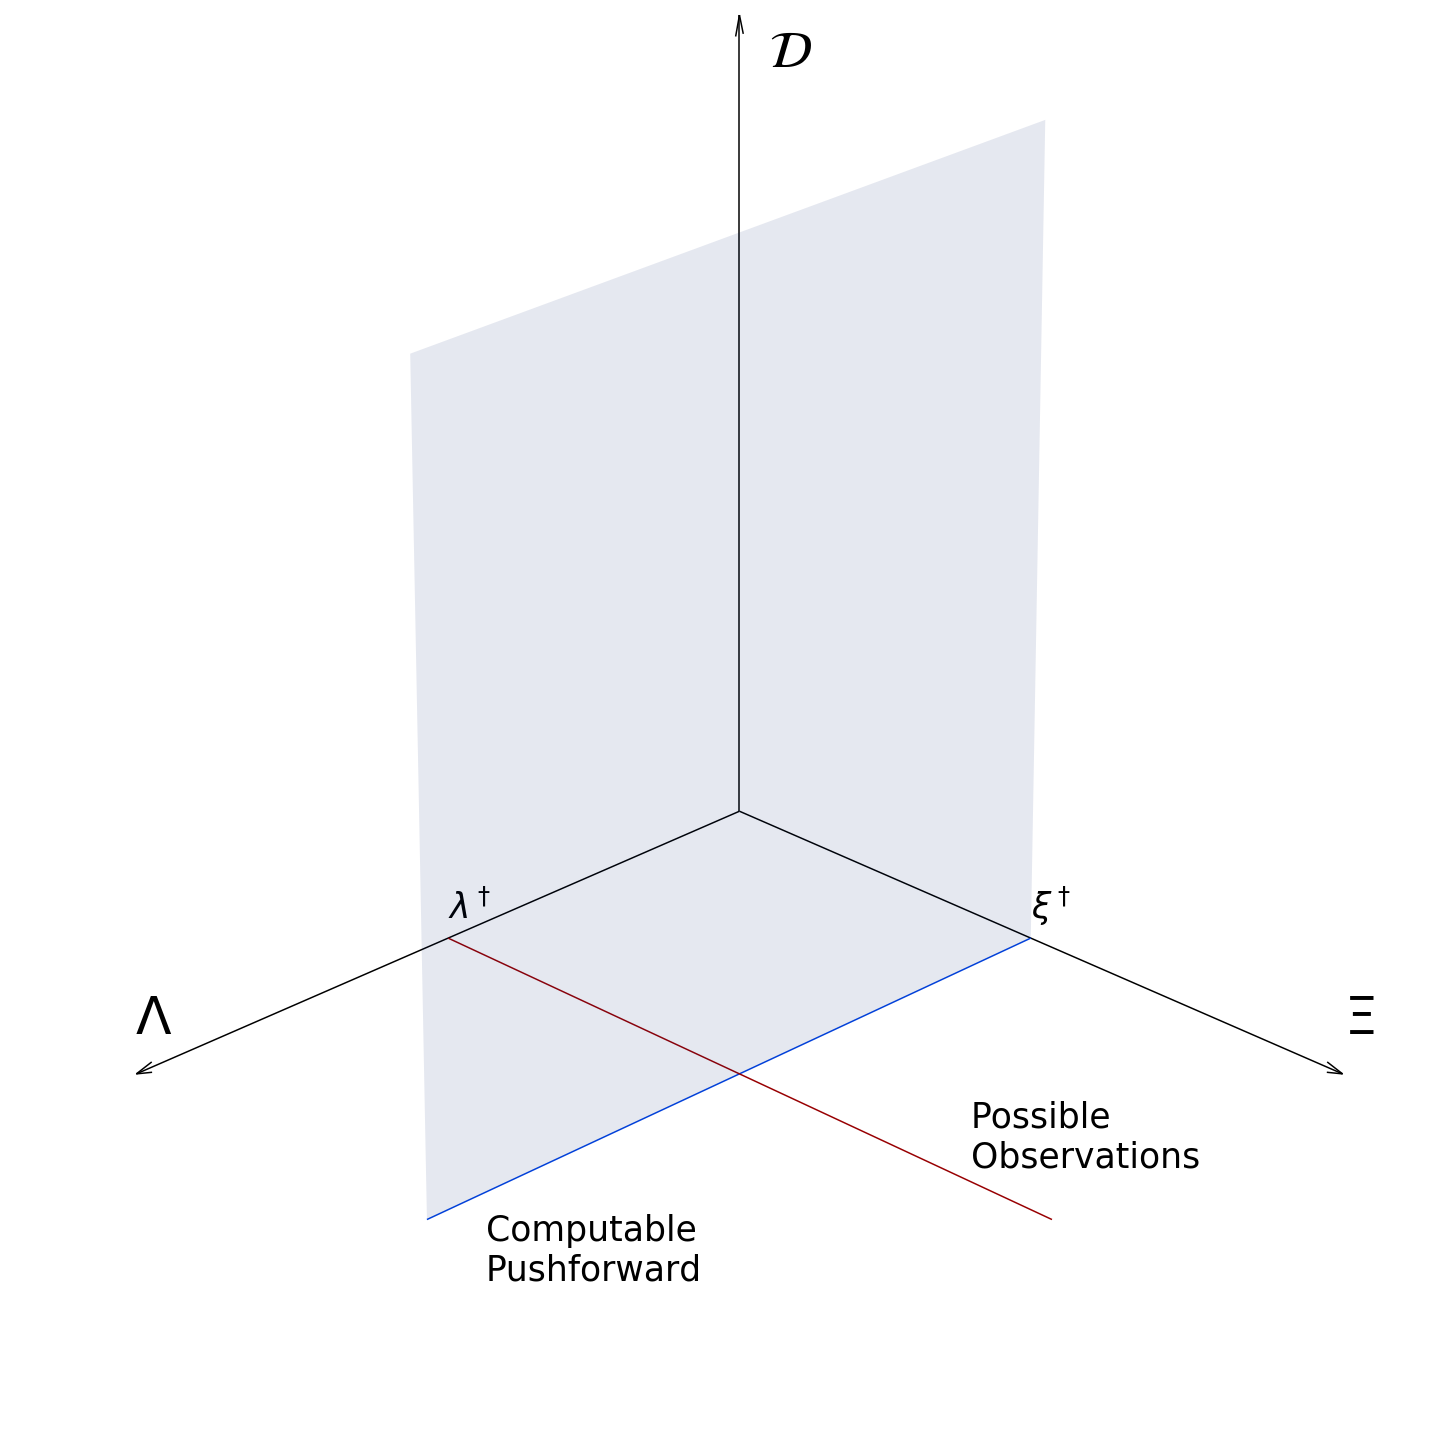
\includegraphics[height=23cm]{diagram}
    \caption*{\large \emph How do conditionals of $\nspace$ compare to the joint density?}
    \end{figure}


\heading{Observed Distribution}
{\large \emph Given a functional, what measure do we invert?}

\Large
    $Q(\param^\dagger, \noise) \sim \observed$ when we allow $\noise$ to vary over $\nspace$
%\vspace{1cm}
    \begin{table}
      \centering
      {\setlength{\tabcolsep}{0.25em}
      \begin{tabular}{c <{\hspace{1pc}} c >{\hspace{1pc}} c}
        %\toprule
        %\large
        \textbf{$F(\obs, \data^\dagger)$} & \textbf{$\noise$} & {$\observed$} \\
        \midrule
        $\frac{1}{\sigma\sqrt{D}} \large\sum \left( \obs_i\lam - \data_i^\dagger \right)$ & $ \noise \sim L^2$ & $N(0,1) $ \\[1.5ex]
        $\frac{1}{\sigma^2} \large\sum \left ( \obs_i\lam - \data_i^\dagger \right)^2$ & $ \noise \sim N(0,\sigma^2) $ & $\chi^2 (D)$ \\[1.5ex]
        $\frac{1}{\sigma^2 D} \large\sum \left ( \obs_i\lam - \data_i^\dagger \right)^2$ & $ \noise \sim N(0,\sigma^2) $ & $ \Gamma \left ( D/2, D/2) \right ) $ \\
        \normalsize\vdots & \normalsize\vdots & \normalsize\vdots \\
        %\bottomrule
      \end{tabular}
      }
      \caption*{Choices of $F$ and associated $\observed$ for stochastic inverse problem}
    \end{table}

%
\end{block}


\end{column}

\separatorcolumn

\begin{column}{\colwidth}

  \begin{block}{Example}
\centering
    Consider an exponential decay problem with uncertain initial condition:
%    \begin{equation*}
%        \partial_t u = - u, \; u(t_0) = \lambda^\dagger = 0.5
%    \end{equation*}
\vspace{-0.5cm}
    \begin{figure}
        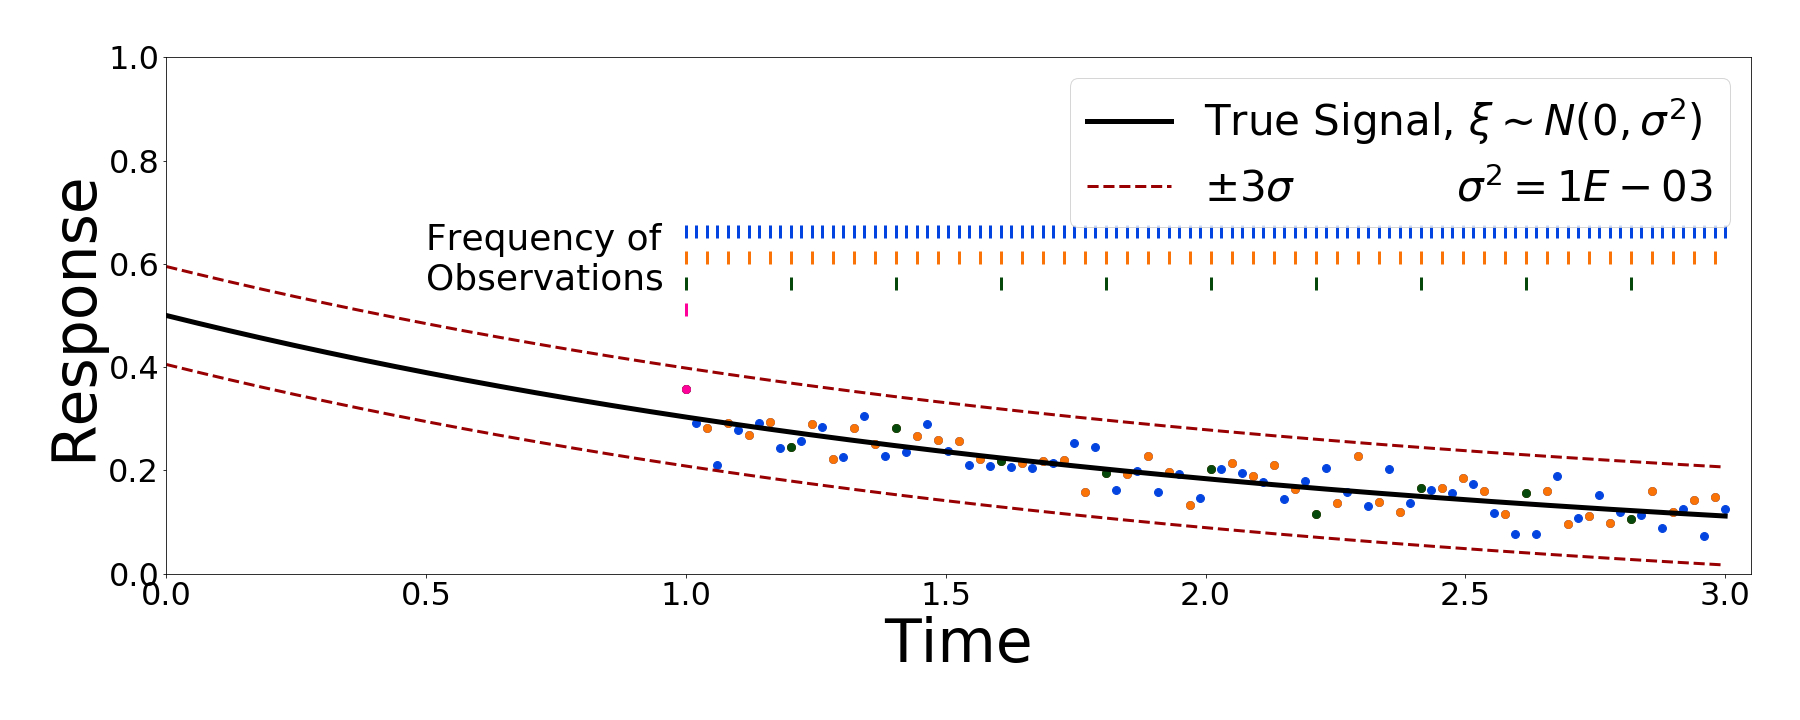
\includegraphics[width=26cm]{exponential_decay_response_sigma-10E-4}
    \end{figure}

%\end{block}

\vspace{1cm}

%\begin{block}{Convergence}
\centering
\heading{\LARGE Convergence}
{\emph How do solutions change with more data?}
\vspace{-0.5cm}
    \begin{figure}
        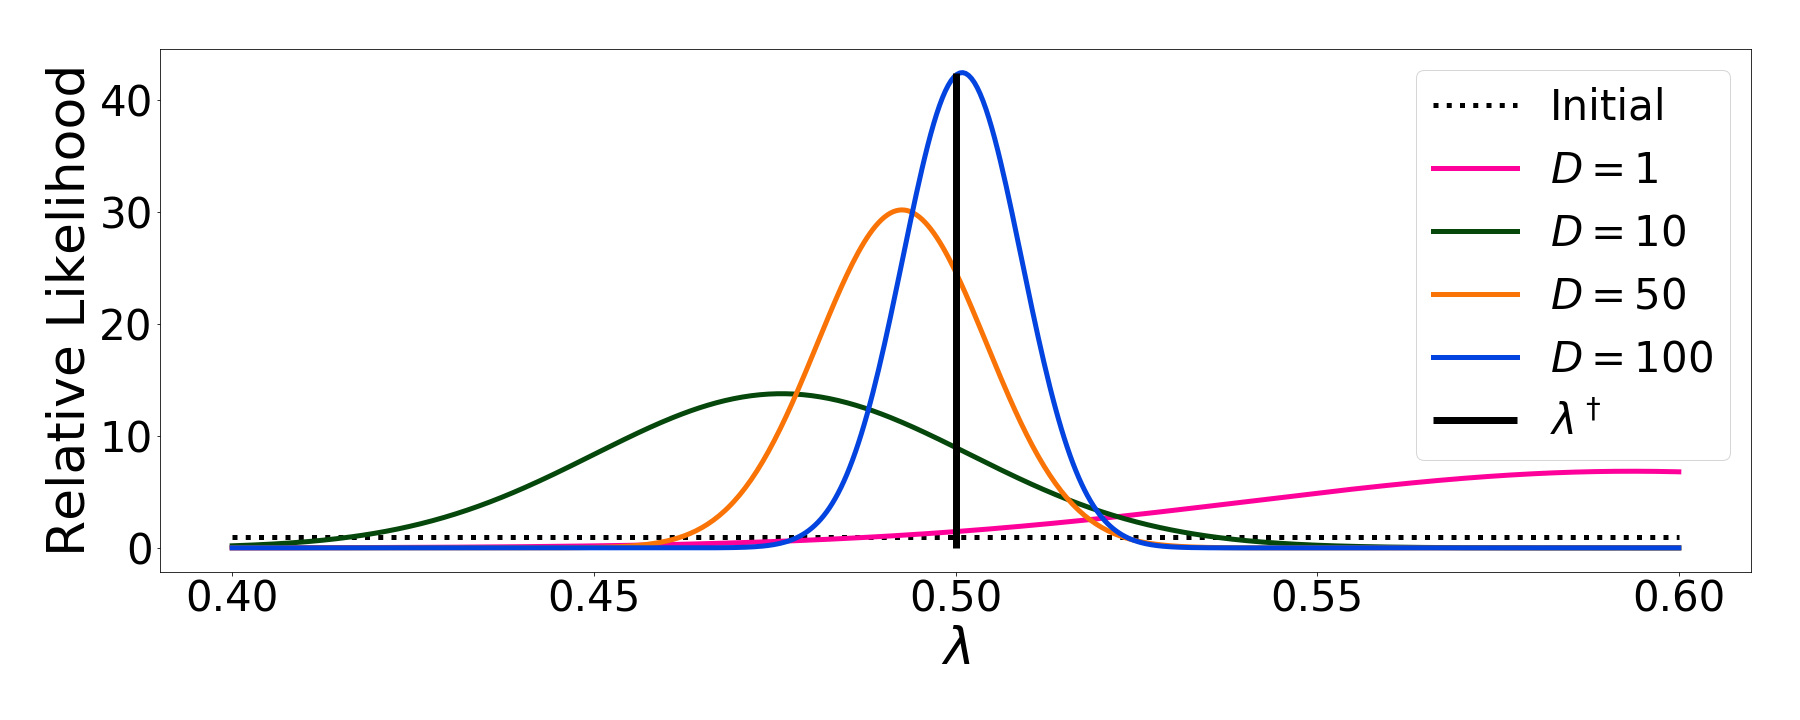
\includegraphics[width=26cm]{updated_convergence_sigma-10E-4}
        \vspace{-0.5cm}
        \caption{ $\param^\dagger$ and $\updated$ for $D=1, 10, 50, 100$ for $N=1000$}
    \end{figure}

%\end{block}

\vspace{1cm}

%\begin{block}{Stability}
\heading{\LARGE Stability}
{\emph How do solutions on conditionals of $\nspace$ compare?}
\vspace{-0.5cm}
    \begin{figure}
        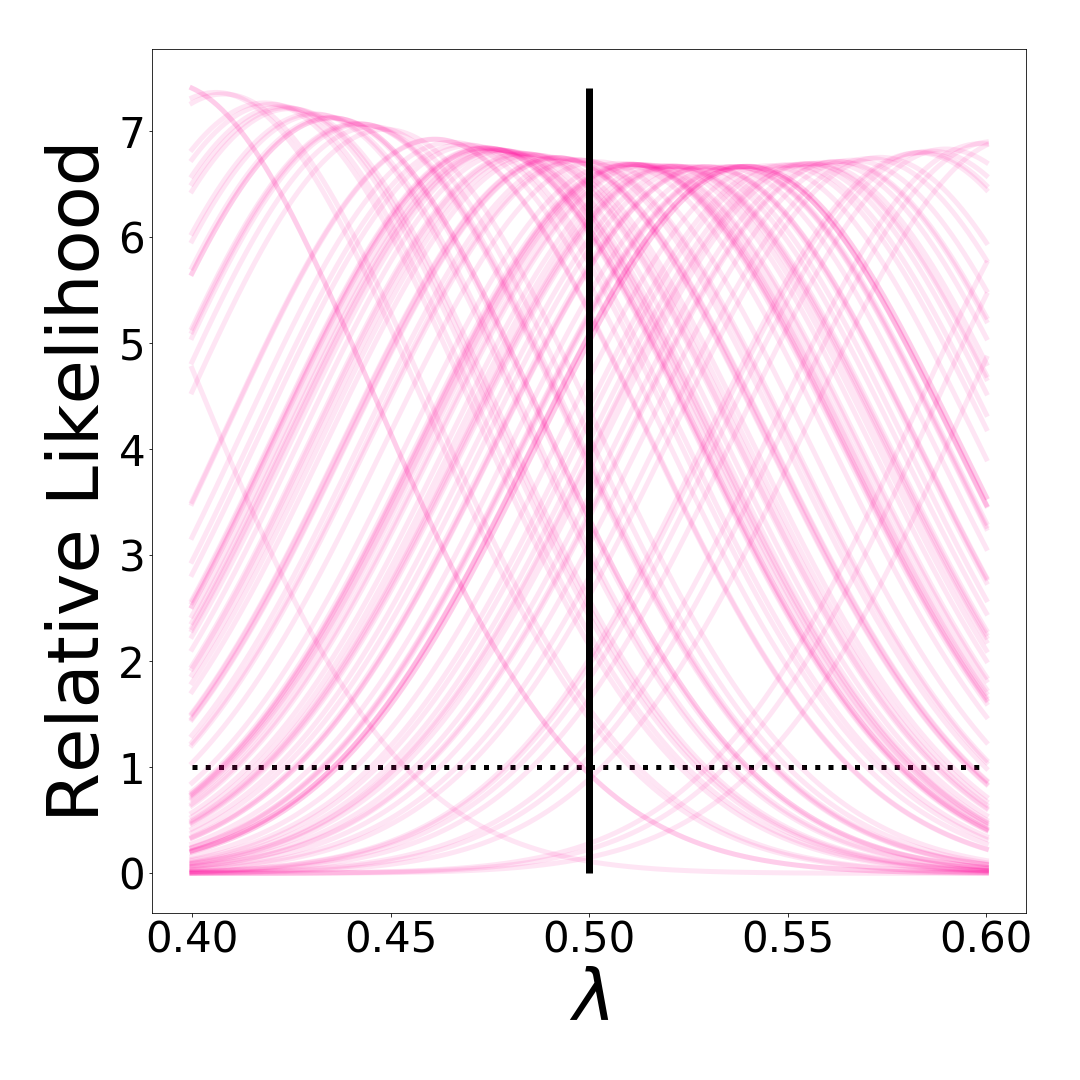
\includegraphics[width=13cm]{updated_stability_D1_sigma-10E-4}
        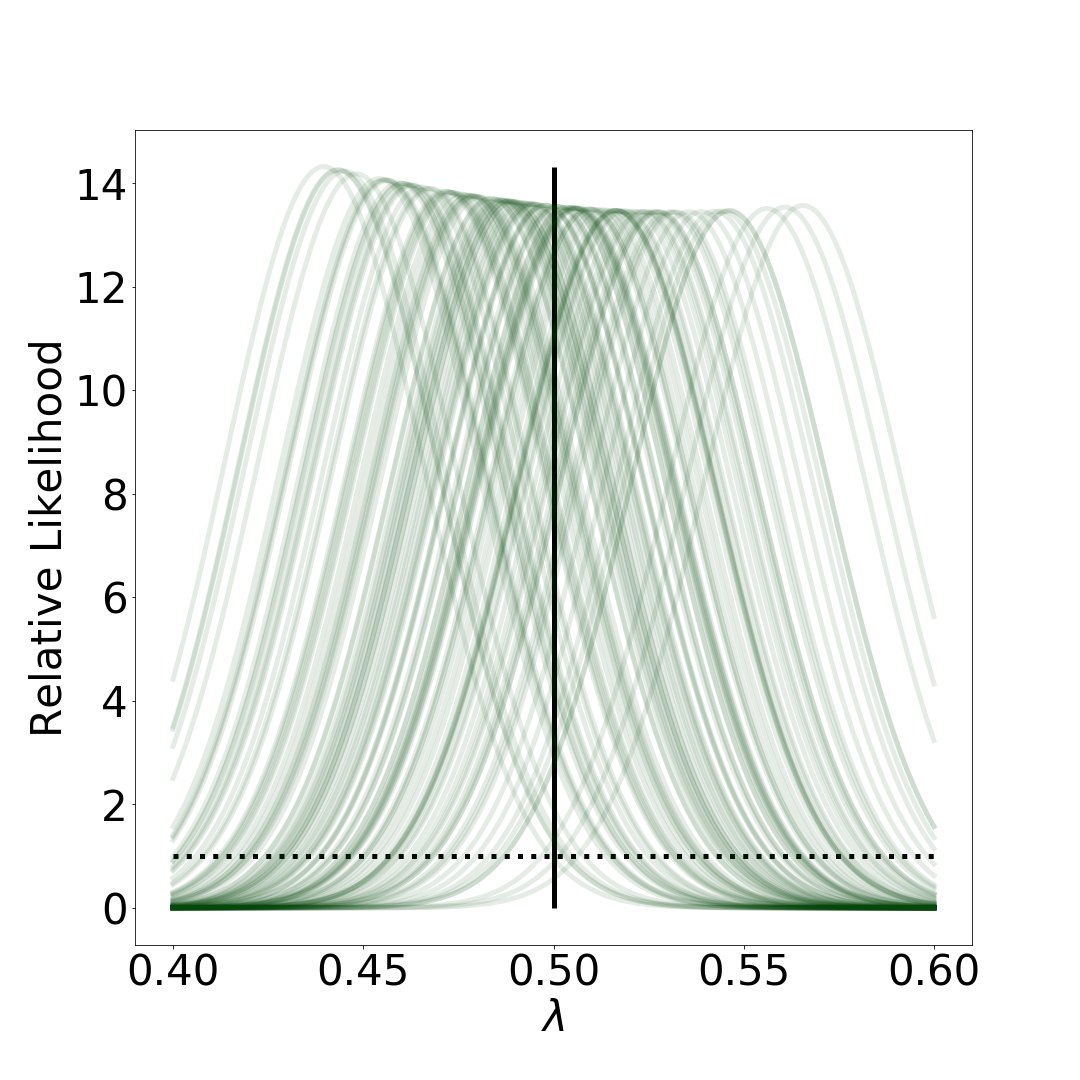
\includegraphics[width=13cm]{updated_stability_D10_sigma-10E-4}\\
        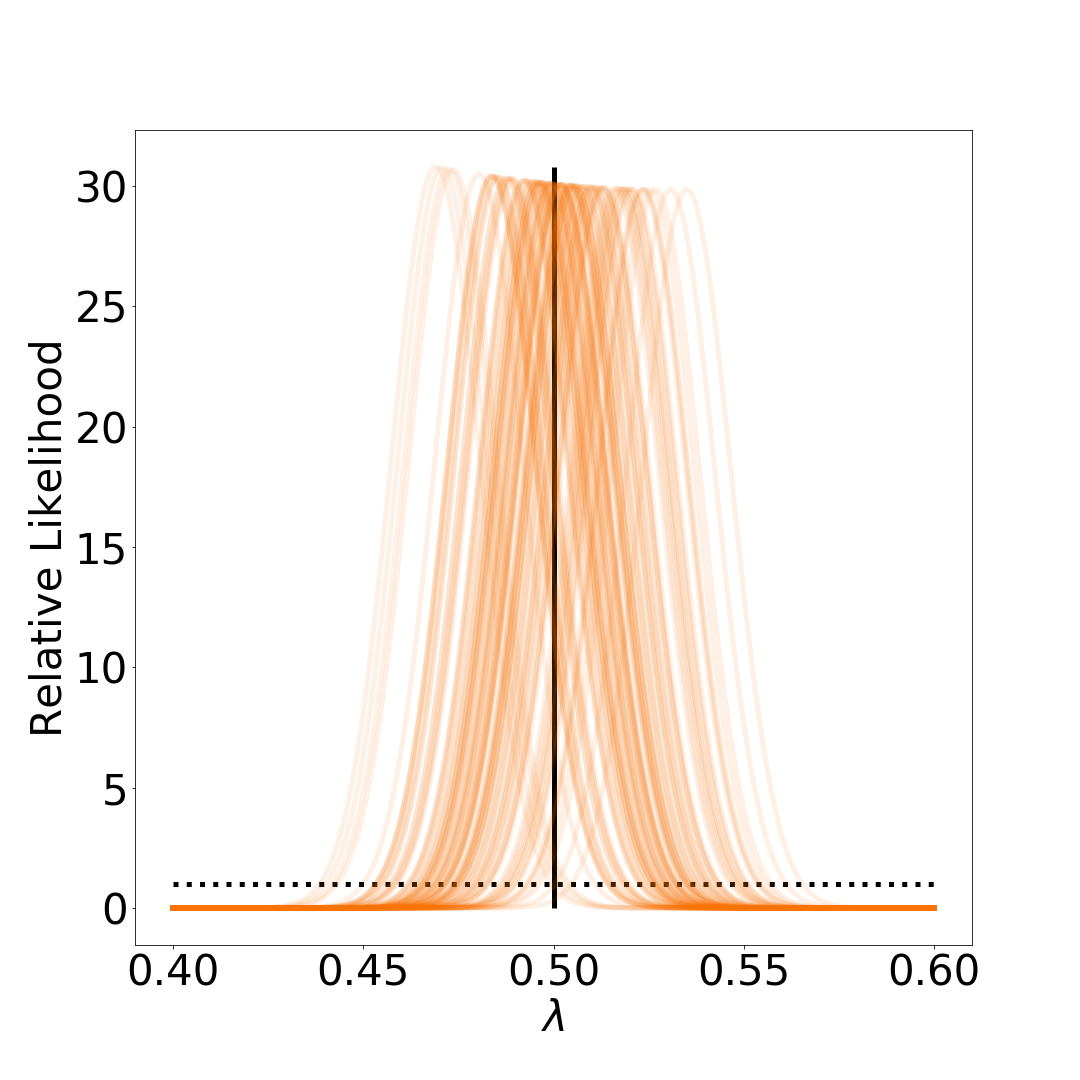
\includegraphics[width=13cm]{updated_stability_D50_sigma-10E-4}
        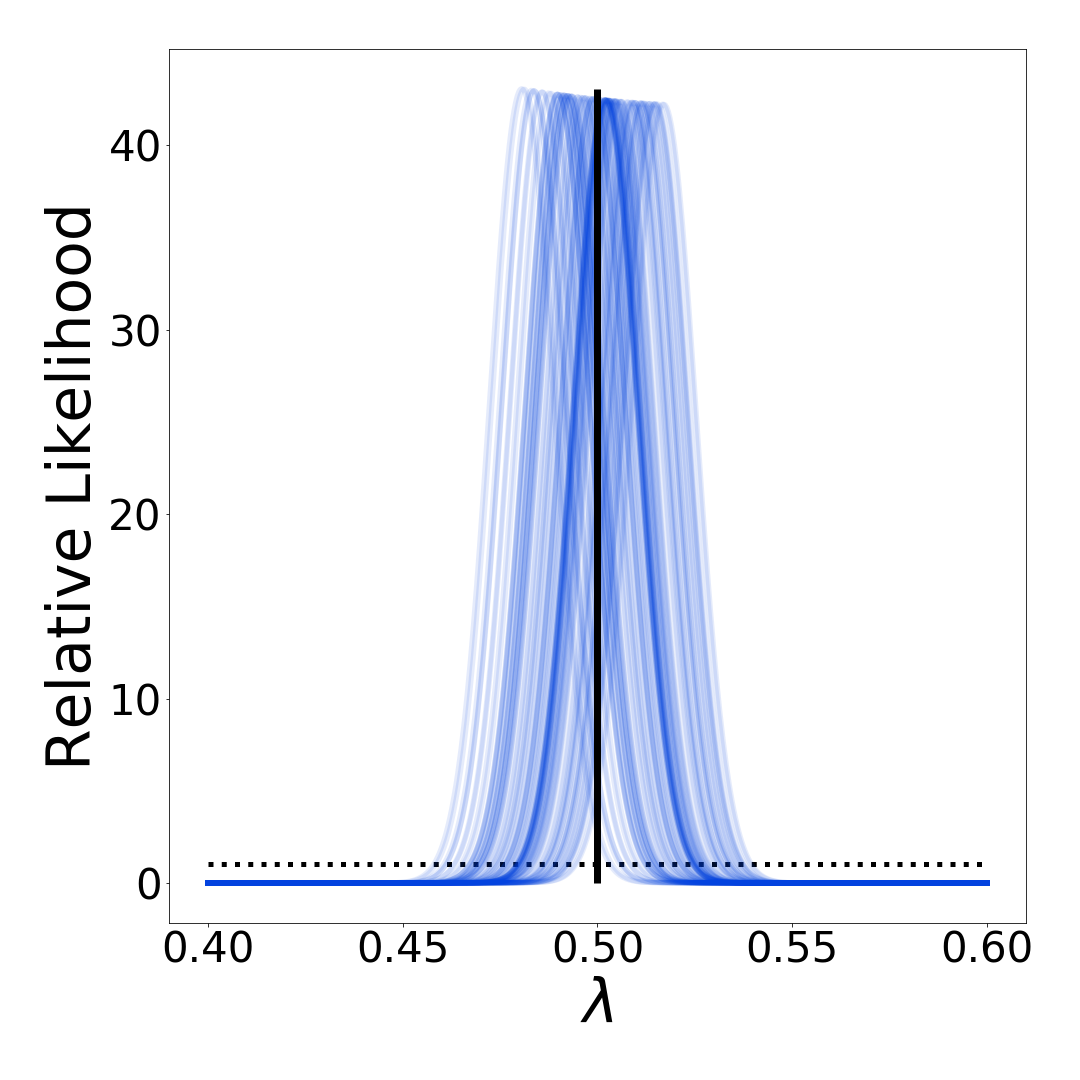
\includegraphics[width=13cm]{updated_stability_D100_sigma-10E-4}
        \vspace{-1cm}
        \caption{$\param^\dagger$ and $\updated$ for one hundred realizations of $\noise^\dagger$ for $D=1, 10, 50, 100$}
    \end{figure}

\end{block}

  
\end{column}

\separatorcolumn
\end{columns}
\end{frame}

\end{document}
